% Created by tikzDevice version 0.7.0 on 2015-01-17 18:10:14
% !TEX encoding = UTF-8 Unicode
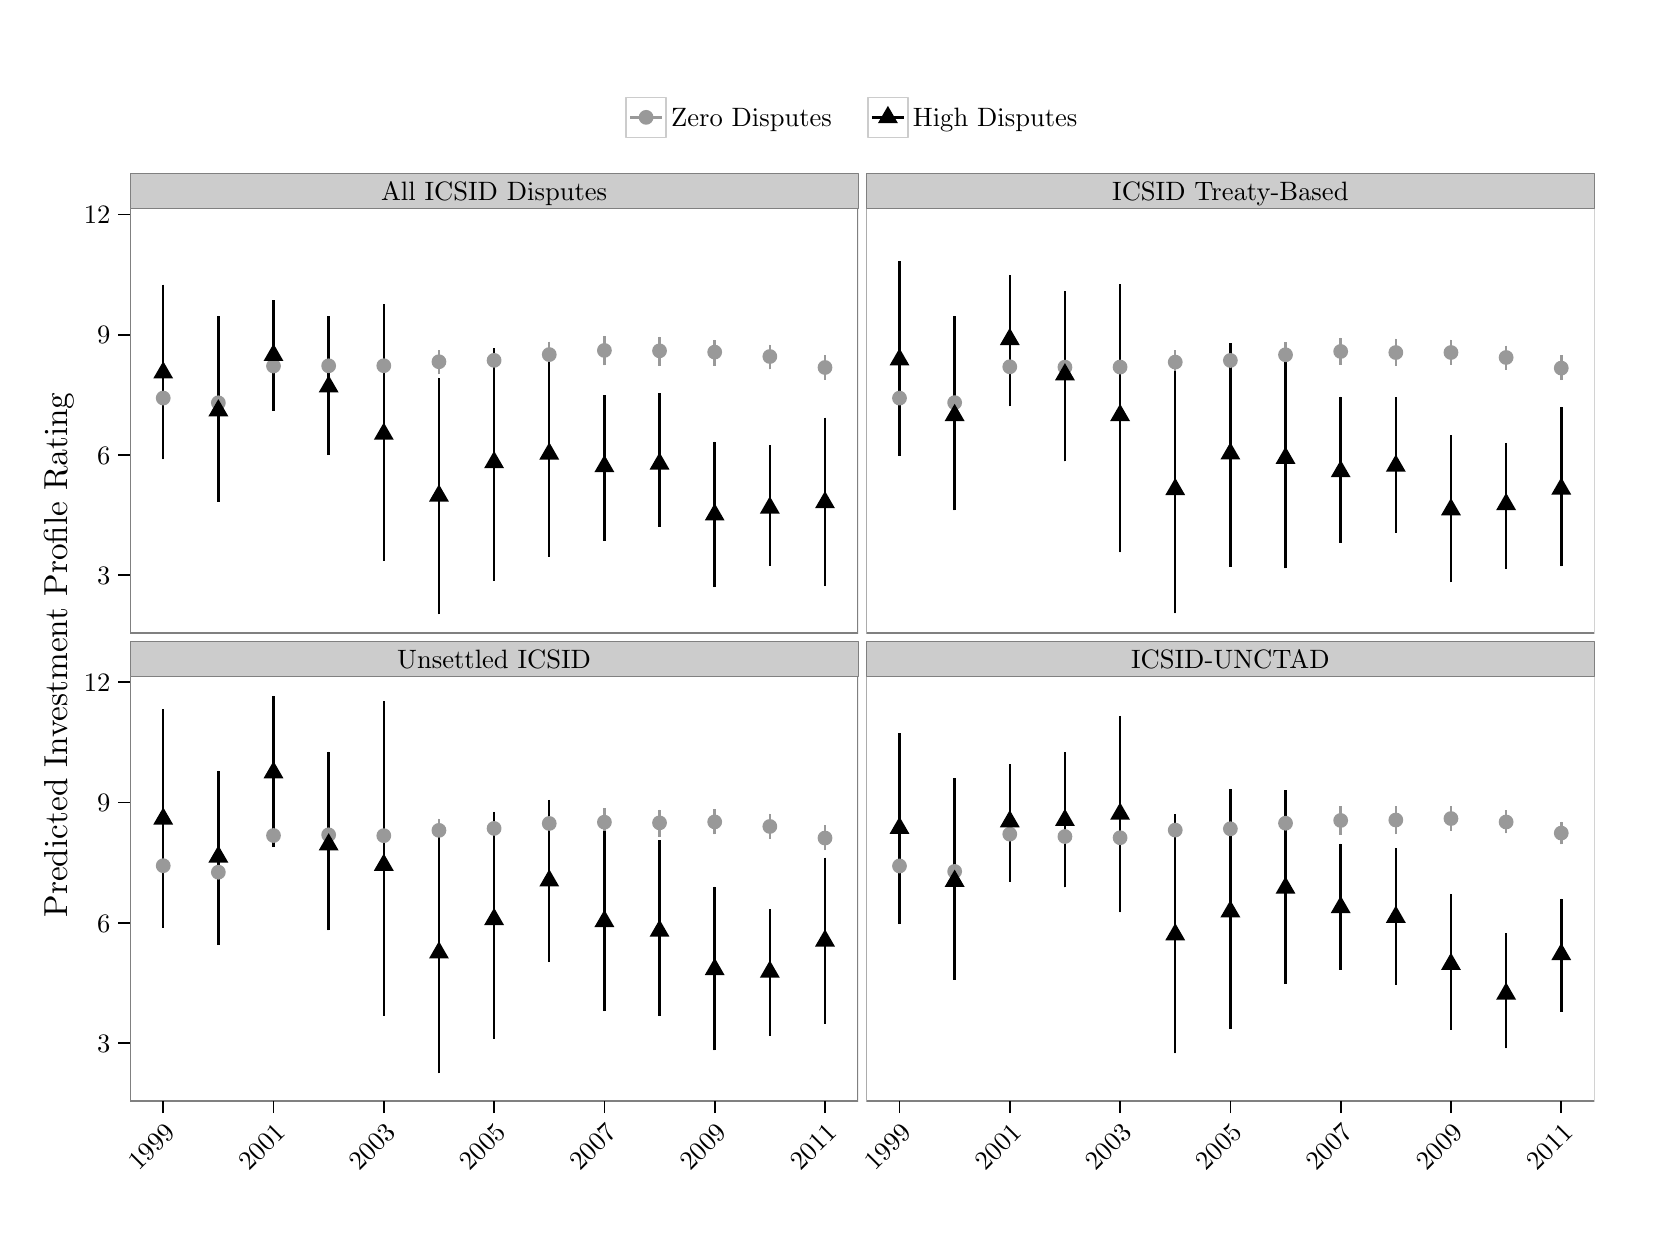
\begin{tikzpicture}[x=1pt,y=1pt]
\definecolor[named]{fillColor}{rgb}{1.00,1.00,1.00}
\path[use as bounding box,fill=fillColor,fill opacity=0.00] (0,0) rectangle (578.16,433.62);
\begin{scope}
\path[clip] (  0.00,  0.00) rectangle (578.16,433.62);
\definecolor[named]{drawColor}{rgb}{1.00,1.00,1.00}
\definecolor[named]{fillColor}{rgb}{1.00,1.00,1.00}

\path[draw=drawColor,line width= 0.6pt,line join=round,line cap=round,fill=fillColor] (  0.00,  0.00) rectangle (578.16,433.62);
\end{scope}
\begin{scope}
\path[clip] ( 37.02,214.77) rectangle (300.06,368.22);
\definecolor[named]{fillColor}{rgb}{1.00,1.00,1.00}

\path[fill=fillColor] ( 37.02,214.77) rectangle (300.06,368.22);
\definecolor[named]{drawColor}{rgb}{0.60,0.60,0.60}
\definecolor[named]{fillColor}{rgb}{0.60,0.60,0.60}

\path[draw=drawColor,line width= 0.9pt,line join=round,fill=fillColor] ( 48.98,293.67) -- ( 48.98,305.59);

\path[draw=drawColor,line width= 0.9pt,line join=round,fill=fillColor] ( 68.90,291.93) -- ( 68.90,304.29);

\path[draw=drawColor,line width= 0.9pt,line join=round,fill=fillColor] ( 88.83,307.70) -- ( 88.83,315.07);

\path[draw=drawColor,line width= 0.9pt,line join=round,fill=fillColor] (108.76,305.93) -- (108.76,317.28);

\path[draw=drawColor,line width= 0.9pt,line join=round,fill=fillColor] (128.69,306.46) -- (128.69,316.72);

\path[draw=drawColor,line width= 0.9pt,line join=round,fill=fillColor] (148.61,308.45) -- (148.61,317.07);

\path[draw=drawColor,line width= 0.9pt,line join=round,fill=fillColor] (168.54,309.24) -- (168.54,317.81);

\path[draw=drawColor,line width= 0.9pt,line join=round,fill=fillColor] (188.47,310.64) -- (188.47,320.16);

\path[draw=drawColor,line width= 0.9pt,line join=round,fill=fillColor] (208.40,311.61) -- (208.40,322.25);

\path[draw=drawColor,line width= 0.9pt,line join=round,fill=fillColor] (228.32,311.45) -- (228.32,321.98);

\path[draw=drawColor,line width= 0.9pt,line join=round,fill=fillColor] (248.25,311.52) -- (248.25,320.82);

\path[draw=drawColor,line width= 0.9pt,line join=round,fill=fillColor] (268.18,310.10) -- (268.18,319.07);

\path[draw=drawColor,line width= 0.9pt,line join=round,fill=fillColor] (288.11,306.38) -- (288.11,315.18);
\definecolor[named]{drawColor}{rgb}{0.00,0.00,0.00}
\definecolor[named]{fillColor}{rgb}{0.00,0.00,0.00}

\path[draw=drawColor,line width= 0.9pt,line join=round,fill=fillColor] ( 48.98,277.65) -- ( 48.98,340.81);

\path[draw=drawColor,line width= 0.9pt,line join=round,fill=fillColor] ( 68.90,262.34) -- ( 68.90,329.49);

\path[draw=drawColor,line width= 0.9pt,line join=round,fill=fillColor] ( 88.83,295.23) -- ( 88.83,335.12);

\path[draw=drawColor,line width= 0.9pt,line join=round,fill=fillColor] (108.76,279.19) -- (108.76,329.36);

\path[draw=drawColor,line width= 0.9pt,line join=round,fill=fillColor] (128.69,240.98) -- (128.69,333.61);

\path[draw=drawColor,line width= 0.9pt,line join=round,fill=fillColor] (148.61,221.74) -- (148.61,307.17);

\path[draw=drawColor,line width= 0.9pt,line join=round,fill=fillColor] (168.54,233.78) -- (168.54,317.86);

\path[draw=drawColor,line width= 0.9pt,line join=round,fill=fillColor] (188.47,242.46) -- (188.47,316.24);

\path[draw=drawColor,line width= 0.9pt,line join=round,fill=fillColor] (208.40,248.30) -- (208.40,300.81);

\path[draw=drawColor,line width= 0.9pt,line join=round,fill=fillColor] (228.32,253.28) -- (228.32,301.49);

\path[draw=drawColor,line width= 0.9pt,line join=round,fill=fillColor] (248.25,231.43) -- (248.25,284.04);

\path[draw=drawColor,line width= 0.9pt,line join=round,fill=fillColor] (268.18,239.20) -- (268.18,282.77);

\path[draw=drawColor,line width= 0.9pt,line join=round,fill=fillColor] (288.11,231.84) -- (288.11,292.68);
\definecolor[named]{fillColor}{rgb}{0.60,0.60,0.60}

\path[fill=fillColor] ( 48.98,299.78) circle (  2.67);
\definecolor[named]{fillColor}{rgb}{0.00,0.00,0.00}

\path[fill=fillColor] ( 48.98,313.08) --
	( 52.57,306.86) --
	( 45.38,306.86) --
	cycle;
\definecolor[named]{fillColor}{rgb}{0.60,0.60,0.60}

\path[fill=fillColor] ( 68.90,298.06) circle (  2.67);
\definecolor[named]{fillColor}{rgb}{0.00,0.00,0.00}

\path[fill=fillColor] ( 68.90,299.40) --
	( 72.50,293.18) --
	( 65.31,293.18) --
	cycle;
\definecolor[named]{fillColor}{rgb}{0.60,0.60,0.60}

\path[fill=fillColor] ( 88.83,311.37) circle (  2.67);
\definecolor[named]{fillColor}{rgb}{0.00,0.00,0.00}

\path[fill=fillColor] ( 88.83,319.41) --
	( 92.42,313.18) --
	( 85.24,313.18) --
	cycle;
\definecolor[named]{fillColor}{rgb}{0.60,0.60,0.60}

\path[fill=fillColor] (108.76,311.43) circle (  2.67);
\definecolor[named]{fillColor}{rgb}{0.00,0.00,0.00}

\path[fill=fillColor] (108.76,308.05) --
	(112.35,301.83) --
	(105.17,301.83) --
	cycle;
\definecolor[named]{fillColor}{rgb}{0.60,0.60,0.60}

\path[fill=fillColor] (128.69,311.46) circle (  2.67);
\definecolor[named]{fillColor}{rgb}{0.00,0.00,0.00}

\path[fill=fillColor] (128.69,290.94) --
	(132.28,284.72) --
	(125.09,284.72) --
	cycle;
\definecolor[named]{fillColor}{rgb}{0.60,0.60,0.60}

\path[fill=fillColor] (148.61,312.90) circle (  2.67);
\definecolor[named]{fillColor}{rgb}{0.00,0.00,0.00}

\path[fill=fillColor] (148.61,268.61) --
	(152.21,262.38) --
	(145.02,262.38) --
	cycle;
\definecolor[named]{fillColor}{rgb}{0.60,0.60,0.60}

\path[fill=fillColor] (168.54,313.40) circle (  2.67);
\definecolor[named]{fillColor}{rgb}{0.00,0.00,0.00}

\path[fill=fillColor] (168.54,280.68) --
	(172.13,274.46) --
	(164.95,274.46) --
	cycle;
\definecolor[named]{fillColor}{rgb}{0.60,0.60,0.60}

\path[fill=fillColor] (188.47,315.49) circle (  2.67);
\definecolor[named]{fillColor}{rgb}{0.00,0.00,0.00}

\path[fill=fillColor] (188.47,283.79) --
	(192.06,277.57) --
	(184.88,277.57) --
	cycle;
\definecolor[named]{fillColor}{rgb}{0.60,0.60,0.60}

\path[fill=fillColor] (208.40,316.99) circle (  2.67);
\definecolor[named]{fillColor}{rgb}{0.00,0.00,0.00}

\path[fill=fillColor] (208.40,279.25) --
	(211.99,273.03) --
	(204.80,273.03) --
	cycle;
\definecolor[named]{fillColor}{rgb}{0.60,0.60,0.60}

\path[fill=fillColor] (228.32,316.84) circle (  2.67);
\definecolor[named]{fillColor}{rgb}{0.00,0.00,0.00}

\path[fill=fillColor] (228.32,280.17) --
	(231.92,273.95) --
	(224.73,273.95) --
	cycle;
\definecolor[named]{fillColor}{rgb}{0.60,0.60,0.60}

\path[fill=fillColor] (248.25,316.38) circle (  2.67);
\definecolor[named]{fillColor}{rgb}{0.00,0.00,0.00}

\path[fill=fillColor] (248.25,261.76) --
	(251.84,255.54) --
	(244.66,255.54) --
	cycle;
\definecolor[named]{fillColor}{rgb}{0.60,0.60,0.60}

\path[fill=fillColor] (268.18,314.79) circle (  2.67);
\definecolor[named]{fillColor}{rgb}{0.00,0.00,0.00}

\path[fill=fillColor] (268.18,264.27) --
	(271.77,258.04) --
	(264.59,258.04) --
	cycle;
\definecolor[named]{fillColor}{rgb}{0.60,0.60,0.60}

\path[fill=fillColor] (288.11,310.83) circle (  2.67);
\definecolor[named]{fillColor}{rgb}{0.00,0.00,0.00}

\path[fill=fillColor] (288.11,266.20) --
	(291.70,259.97) --
	(284.51,259.97) --
	cycle;
\definecolor[named]{drawColor}{rgb}{0.50,0.50,0.50}

\path[draw=drawColor,line width= 0.6pt,line join=round,line cap=round] ( 37.02,214.77) rectangle (300.06,368.22);
\end{scope}
\begin{scope}
\path[clip] (303.07,214.77) rectangle (566.12,368.22);
\definecolor[named]{fillColor}{rgb}{1.00,1.00,1.00}

\path[fill=fillColor] (303.07,214.77) rectangle (566.12,368.22);
\definecolor[named]{drawColor}{rgb}{0.60,0.60,0.60}
\definecolor[named]{fillColor}{rgb}{0.60,0.60,0.60}

\path[draw=drawColor,line width= 0.9pt,line join=round,fill=fillColor] (315.03,293.78) -- (315.03,305.84);

\path[draw=drawColor,line width= 0.9pt,line join=round,fill=fillColor] (334.96,291.95) -- (334.96,304.13);

\path[draw=drawColor,line width= 0.9pt,line join=round,fill=fillColor] (354.88,307.16) -- (354.88,314.84);

\path[draw=drawColor,line width= 0.9pt,line join=round,fill=fillColor] (374.81,305.98) -- (374.81,316.10);

\path[draw=drawColor,line width= 0.9pt,line join=round,fill=fillColor] (394.74,305.73) -- (394.74,316.18);

\path[draw=drawColor,line width= 0.9pt,line join=round,fill=fillColor] (414.67,308.47) -- (414.67,316.99);

\path[draw=drawColor,line width= 0.9pt,line join=round,fill=fillColor] (434.59,309.08) -- (434.59,317.58);

\path[draw=drawColor,line width= 0.9pt,line join=round,fill=fillColor] (454.52,310.77) -- (454.52,319.96);

\path[draw=drawColor,line width= 0.9pt,line join=round,fill=fillColor] (474.45,311.76) -- (474.45,321.65);

\path[draw=drawColor,line width= 0.9pt,line join=round,fill=fillColor] (494.38,311.49) -- (494.38,321.25);

\path[draw=drawColor,line width= 0.9pt,line join=round,fill=fillColor] (514.30,311.80) -- (514.30,320.87);

\path[draw=drawColor,line width= 0.9pt,line join=round,fill=fillColor] (534.23,310.00) -- (534.23,318.75);

\path[draw=drawColor,line width= 0.9pt,line join=round,fill=fillColor] (554.16,306.27) -- (554.16,315.18);
\definecolor[named]{drawColor}{rgb}{0.00,0.00,0.00}
\definecolor[named]{fillColor}{rgb}{0.00,0.00,0.00}

\path[draw=drawColor,line width= 0.9pt,line join=round,fill=fillColor] (315.03,278.99) -- (315.03,349.30);

\path[draw=drawColor,line width= 0.9pt,line join=round,fill=fillColor] (334.96,259.18) -- (334.96,329.45);

\path[draw=drawColor,line width= 0.9pt,line join=round,fill=fillColor] (354.88,296.83) -- (354.88,344.32);

\path[draw=drawColor,line width= 0.9pt,line join=round,fill=fillColor] (374.81,276.90) -- (374.81,338.49);

\path[draw=drawColor,line width= 0.9pt,line join=round,fill=fillColor] (394.74,243.99) -- (394.74,340.82);

\path[draw=drawColor,line width= 0.9pt,line join=round,fill=fillColor] (414.67,221.97) -- (414.67,309.69);

\path[draw=drawColor,line width= 0.9pt,line join=round,fill=fillColor] (434.59,238.83) -- (434.59,319.61);

\path[draw=drawColor,line width= 0.9pt,line join=round,fill=fillColor] (454.52,238.22) -- (454.52,316.91);

\path[draw=drawColor,line width= 0.9pt,line join=round,fill=fillColor] (474.45,247.41) -- (474.45,300.28);

\path[draw=drawColor,line width= 0.9pt,line join=round,fill=fillColor] (494.38,251.06) -- (494.38,300.07);

\path[draw=drawColor,line width= 0.9pt,line join=round,fill=fillColor] (514.30,233.31) -- (514.30,286.29);

\path[draw=drawColor,line width= 0.9pt,line join=round,fill=fillColor] (534.23,238.00) -- (534.23,283.55);

\path[draw=drawColor,line width= 0.9pt,line join=round,fill=fillColor] (554.16,238.96) -- (554.16,296.55);
\definecolor[named]{fillColor}{rgb}{0.60,0.60,0.60}

\path[fill=fillColor] (315.03,299.76) circle (  2.67);
\definecolor[named]{fillColor}{rgb}{0.00,0.00,0.00}

\path[fill=fillColor] (315.03,317.80) --
	(318.62,311.58) --
	(311.44,311.58) --
	cycle;
\definecolor[named]{fillColor}{rgb}{0.60,0.60,0.60}

\path[fill=fillColor] (334.96,298.12) circle (  2.67);
\definecolor[named]{fillColor}{rgb}{0.00,0.00,0.00}

\path[fill=fillColor] (334.96,297.70) --
	(338.55,291.48) --
	(331.36,291.48) --
	cycle;
\definecolor[named]{fillColor}{rgb}{0.60,0.60,0.60}

\path[fill=fillColor] (354.88,311.08) circle (  2.67);
\definecolor[named]{fillColor}{rgb}{0.00,0.00,0.00}

\path[fill=fillColor] (354.88,325.15) --
	(358.48,318.92) --
	(351.29,318.92) --
	cycle;
\definecolor[named]{fillColor}{rgb}{0.60,0.60,0.60}

\path[fill=fillColor] (374.81,310.94) circle (  2.67);
\definecolor[named]{fillColor}{rgb}{0.00,0.00,0.00}

\path[fill=fillColor] (374.81,312.41) --
	(378.40,306.19) --
	(371.22,306.19) --
	cycle;
\definecolor[named]{fillColor}{rgb}{0.60,0.60,0.60}

\path[fill=fillColor] (394.74,310.98) circle (  2.67);
\definecolor[named]{fillColor}{rgb}{0.00,0.00,0.00}

\path[fill=fillColor] (394.74,297.69) --
	(398.33,291.47) --
	(391.15,291.47) --
	cycle;
\definecolor[named]{fillColor}{rgb}{0.60,0.60,0.60}

\path[fill=fillColor] (414.67,312.77) circle (  2.67);
\definecolor[named]{fillColor}{rgb}{0.00,0.00,0.00}

\path[fill=fillColor] (414.67,270.93) --
	(418.26,264.71) --
	(411.07,264.71) --
	cycle;
\definecolor[named]{fillColor}{rgb}{0.60,0.60,0.60}

\path[fill=fillColor] (434.59,313.37) circle (  2.67);
\definecolor[named]{fillColor}{rgb}{0.00,0.00,0.00}

\path[fill=fillColor] (434.59,283.82) --
	(438.19,277.59) --
	(431.00,277.59) --
	cycle;
\definecolor[named]{fillColor}{rgb}{0.60,0.60,0.60}

\path[fill=fillColor] (454.52,315.42) circle (  2.67);
\definecolor[named]{fillColor}{rgb}{0.00,0.00,0.00}

\path[fill=fillColor] (454.52,282.24) --
	(458.11,276.02) --
	(450.93,276.02) --
	cycle;
\definecolor[named]{fillColor}{rgb}{0.60,0.60,0.60}

\path[fill=fillColor] (474.45,316.62) circle (  2.67);
\definecolor[named]{fillColor}{rgb}{0.00,0.00,0.00}

\path[fill=fillColor] (474.45,277.40) --
	(478.04,271.18) --
	(470.86,271.18) --
	cycle;
\definecolor[named]{fillColor}{rgb}{0.60,0.60,0.60}

\path[fill=fillColor] (494.38,316.22) circle (  2.67);
\definecolor[named]{fillColor}{rgb}{0.00,0.00,0.00}

\path[fill=fillColor] (494.38,279.40) --
	(497.97,273.18) --
	(490.78,273.18) --
	cycle;
\definecolor[named]{fillColor}{rgb}{0.60,0.60,0.60}

\path[fill=fillColor] (514.30,316.24) circle (  2.67);
\definecolor[named]{fillColor}{rgb}{0.00,0.00,0.00}

\path[fill=fillColor] (514.30,263.64) --
	(517.90,257.42) --
	(510.71,257.42) --
	cycle;
\definecolor[named]{fillColor}{rgb}{0.60,0.60,0.60}

\path[fill=fillColor] (534.23,314.44) circle (  2.67);
\definecolor[named]{fillColor}{rgb}{0.00,0.00,0.00}

\path[fill=fillColor] (534.23,265.53) --
	(537.82,259.31) --
	(530.64,259.31) --
	cycle;
\definecolor[named]{fillColor}{rgb}{0.60,0.60,0.60}

\path[fill=fillColor] (554.16,310.60) circle (  2.67);
\definecolor[named]{fillColor}{rgb}{0.00,0.00,0.00}

\path[fill=fillColor] (554.16,271.14) --
	(557.75,264.92) --
	(550.57,264.92) --
	cycle;
\definecolor[named]{drawColor}{rgb}{0.50,0.50,0.50}

\path[draw=drawColor,line width= 0.6pt,line join=round,line cap=round] (303.07,214.77) rectangle (566.12,368.22);
\end{scope}
\begin{scope}
\path[clip] ( 37.02, 45.67) rectangle (300.06,199.12);
\definecolor[named]{fillColor}{rgb}{1.00,1.00,1.00}

\path[fill=fillColor] ( 37.02, 45.67) rectangle (300.06,199.12);
\definecolor[named]{drawColor}{rgb}{0.60,0.60,0.60}
\definecolor[named]{fillColor}{rgb}{0.60,0.60,0.60}

\path[draw=drawColor,line width= 0.9pt,line join=round,fill=fillColor] ( 48.98,125.38) -- ( 48.98,136.64);

\path[draw=drawColor,line width= 0.9pt,line join=round,fill=fillColor] ( 68.90,122.62) -- ( 68.90,134.68);

\path[draw=drawColor,line width= 0.9pt,line join=round,fill=fillColor] ( 88.83,137.99) -- ( 88.83,145.38);

\path[draw=drawColor,line width= 0.9pt,line join=round,fill=fillColor] (108.76,136.92) -- (108.76,146.80);

\path[draw=drawColor,line width= 0.9pt,line join=round,fill=fillColor] (128.69,136.43) -- (128.69,146.97);

\path[draw=drawColor,line width= 0.9pt,line join=round,fill=fillColor] (148.61,139.21) -- (148.61,147.84);

\path[draw=drawColor,line width= 0.9pt,line join=round,fill=fillColor] (168.54,139.98) -- (168.54,148.92);

\path[draw=drawColor,line width= 0.9pt,line join=round,fill=fillColor] (188.47,141.35) -- (188.47,150.56);

\path[draw=drawColor,line width= 0.9pt,line join=round,fill=fillColor] (208.40,141.52) -- (208.40,151.53);

\path[draw=drawColor,line width= 0.9pt,line join=round,fill=fillColor] (228.32,141.08) -- (228.32,151.10);

\path[draw=drawColor,line width= 0.9pt,line join=round,fill=fillColor] (248.25,142.10) -- (248.25,151.31);

\path[draw=drawColor,line width= 0.9pt,line join=round,fill=fillColor] (268.18,140.56) -- (268.18,149.61);

\path[draw=drawColor,line width= 0.9pt,line join=round,fill=fillColor] (288.11,136.44) -- (288.11,145.36);
\definecolor[named]{drawColor}{rgb}{0.00,0.00,0.00}
\definecolor[named]{fillColor}{rgb}{0.00,0.00,0.00}

\path[draw=drawColor,line width= 0.9pt,line join=round,fill=fillColor] ( 48.98,108.37) -- ( 48.98,187.25);

\path[draw=drawColor,line width= 0.9pt,line join=round,fill=fillColor] ( 68.90,102.13) -- ( 68.90,165.18);

\path[draw=drawColor,line width= 0.9pt,line join=round,fill=fillColor] ( 88.83,137.47) -- ( 88.83,192.15);

\path[draw=drawColor,line width= 0.9pt,line join=round,fill=fillColor] (108.76,107.39) -- (108.76,171.99);

\path[draw=drawColor,line width= 0.9pt,line join=round,fill=fillColor] (128.69, 76.50) -- (128.69,190.14);

\path[draw=drawColor,line width= 0.9pt,line join=round,fill=fillColor] (148.61, 55.81) -- (148.61,142.68);

\path[draw=drawColor,line width= 0.9pt,line join=round,fill=fillColor] (168.54, 68.20) -- (168.54,150.27);

\path[draw=drawColor,line width= 0.9pt,line join=round,fill=fillColor] (188.47, 95.95) -- (188.47,154.62);

\path[draw=drawColor,line width= 0.9pt,line join=round,fill=fillColor] (208.40, 78.21) -- (208.40,143.42);

\path[draw=drawColor,line width= 0.9pt,line join=round,fill=fillColor] (228.32, 76.53) -- (228.32,140.01);

\path[draw=drawColor,line width= 0.9pt,line join=round,fill=fillColor] (248.25, 64.08) -- (248.25,123.27);

\path[draw=drawColor,line width= 0.9pt,line join=round,fill=fillColor] (268.18, 69.38) -- (268.18,115.03);

\path[draw=drawColor,line width= 0.9pt,line join=round,fill=fillColor] (288.11, 73.63) -- (288.11,133.71);
\definecolor[named]{fillColor}{rgb}{0.60,0.60,0.60}

\path[fill=fillColor] ( 48.98,130.79) circle (  2.67);
\definecolor[named]{fillColor}{rgb}{0.00,0.00,0.00}

\path[fill=fillColor] ( 48.98,151.88) --
	( 52.57,145.66) --
	( 45.38,145.66) --
	cycle;
\definecolor[named]{fillColor}{rgb}{0.60,0.60,0.60}

\path[fill=fillColor] ( 68.90,128.45) circle (  2.67);
\definecolor[named]{fillColor}{rgb}{0.00,0.00,0.00}

\path[fill=fillColor] ( 68.90,138.16) --
	( 72.50,131.93) --
	( 65.31,131.93) --
	cycle;
\definecolor[named]{fillColor}{rgb}{0.60,0.60,0.60}

\path[fill=fillColor] ( 88.83,141.70) circle (  2.67);
\definecolor[named]{fillColor}{rgb}{0.00,0.00,0.00}

\path[fill=fillColor] ( 88.83,168.61) --
	( 92.42,162.39) --
	( 85.24,162.39) --
	cycle;
\definecolor[named]{fillColor}{rgb}{0.60,0.60,0.60}

\path[fill=fillColor] (108.76,141.95) circle (  2.67);
\definecolor[named]{fillColor}{rgb}{0.00,0.00,0.00}

\path[fill=fillColor] (108.76,142.56) --
	(112.35,136.34) --
	(105.17,136.34) --
	cycle;
\definecolor[named]{fillColor}{rgb}{0.60,0.60,0.60}

\path[fill=fillColor] (128.69,141.65) circle (  2.67);
\definecolor[named]{fillColor}{rgb}{0.00,0.00,0.00}

\path[fill=fillColor] (128.69,135.19) --
	(132.28,128.97) --
	(125.09,128.97) --
	cycle;
\definecolor[named]{fillColor}{rgb}{0.60,0.60,0.60}

\path[fill=fillColor] (148.61,143.57) circle (  2.67);
\definecolor[named]{fillColor}{rgb}{0.00,0.00,0.00}

\path[fill=fillColor] (148.61,103.50) --
	(152.21, 97.28) --
	(145.02, 97.28) --
	cycle;
\definecolor[named]{fillColor}{rgb}{0.60,0.60,0.60}

\path[fill=fillColor] (168.54,144.27) circle (  2.67);
\definecolor[named]{fillColor}{rgb}{0.00,0.00,0.00}

\path[fill=fillColor] (168.54,115.58) --
	(172.13,109.36) --
	(164.95,109.36) --
	cycle;
\definecolor[named]{fillColor}{rgb}{0.60,0.60,0.60}

\path[fill=fillColor] (188.47,146.06) circle (  2.67);
\definecolor[named]{fillColor}{rgb}{0.00,0.00,0.00}

\path[fill=fillColor] (188.47,129.51) --
	(192.06,123.29) --
	(184.88,123.29) --
	cycle;
\definecolor[named]{fillColor}{rgb}{0.60,0.60,0.60}

\path[fill=fillColor] (208.40,146.52) circle (  2.67);
\definecolor[named]{fillColor}{rgb}{0.00,0.00,0.00}

\path[fill=fillColor] (208.40,114.87) --
	(211.99,108.64) --
	(204.80,108.64) --
	cycle;
\definecolor[named]{fillColor}{rgb}{0.60,0.60,0.60}

\path[fill=fillColor] (228.32,146.28) circle (  2.67);
\definecolor[named]{fillColor}{rgb}{0.00,0.00,0.00}

\path[fill=fillColor] (228.32,111.36) --
	(231.92,105.14) --
	(224.73,105.14) --
	cycle;
\definecolor[named]{fillColor}{rgb}{0.60,0.60,0.60}

\path[fill=fillColor] (248.25,146.63) circle (  2.67);
\definecolor[named]{fillColor}{rgb}{0.00,0.00,0.00}

\path[fill=fillColor] (248.25, 97.50) --
	(251.84, 91.27) --
	(244.66, 91.27) --
	cycle;
\definecolor[named]{fillColor}{rgb}{0.60,0.60,0.60}

\path[fill=fillColor] (268.18,144.98) circle (  2.67);
\definecolor[named]{fillColor}{rgb}{0.00,0.00,0.00}

\path[fill=fillColor] (268.18, 96.58) --
	(271.77, 90.36) --
	(264.59, 90.36) --
	cycle;
\definecolor[named]{fillColor}{rgb}{0.60,0.60,0.60}

\path[fill=fillColor] (288.11,140.79) circle (  2.67);
\definecolor[named]{fillColor}{rgb}{0.00,0.00,0.00}

\path[fill=fillColor] (288.11,107.82) --
	(291.70,101.60) --
	(284.51,101.60) --
	cycle;
\definecolor[named]{drawColor}{rgb}{0.50,0.50,0.50}

\path[draw=drawColor,line width= 0.6pt,line join=round,line cap=round] ( 37.02, 45.67) rectangle (300.06,199.12);
\end{scope}
\begin{scope}
\path[clip] (303.07, 45.67) rectangle (566.12,199.12);
\definecolor[named]{fillColor}{rgb}{1.00,1.00,1.00}

\path[fill=fillColor] (303.07, 45.67) rectangle (566.12,199.12);
\definecolor[named]{drawColor}{rgb}{0.60,0.60,0.60}
\definecolor[named]{fillColor}{rgb}{0.60,0.60,0.60}

\path[draw=drawColor,line width= 0.9pt,line join=round,fill=fillColor] (315.03,124.77) -- (315.03,136.40);

\path[draw=drawColor,line width= 0.9pt,line join=round,fill=fillColor] (334.96,122.55) -- (334.96,134.49);

\path[draw=drawColor,line width= 0.9pt,line join=round,fill=fillColor] (354.88,138.58) -- (354.88,146.09);

\path[draw=drawColor,line width= 0.9pt,line join=round,fill=fillColor] (374.81,135.46) -- (374.81,146.59);

\path[draw=drawColor,line width= 0.9pt,line join=round,fill=fillColor] (394.74,135.88) -- (394.74,145.95);

\path[draw=drawColor,line width= 0.9pt,line join=round,fill=fillColor] (414.67,139.39) -- (414.67,147.97);

\path[draw=drawColor,line width= 0.9pt,line join=round,fill=fillColor] (434.59,139.78) -- (434.59,148.45);

\path[draw=drawColor,line width= 0.9pt,line join=round,fill=fillColor] (454.52,141.53) -- (454.52,150.88);

\path[draw=drawColor,line width= 0.9pt,line join=round,fill=fillColor] (474.45,141.91) -- (474.45,152.29);

\path[draw=drawColor,line width= 0.9pt,line join=round,fill=fillColor] (494.38,142.20) -- (494.38,152.36);

\path[draw=drawColor,line width= 0.9pt,line join=round,fill=fillColor] (514.30,143.35) -- (514.30,152.28);

\path[draw=drawColor,line width= 0.9pt,line join=round,fill=fillColor] (534.23,142.45) -- (534.23,150.85);

\path[draw=drawColor,line width= 0.9pt,line join=round,fill=fillColor] (554.16,138.48) -- (554.16,146.68);
\definecolor[named]{drawColor}{rgb}{0.00,0.00,0.00}
\definecolor[named]{fillColor}{rgb}{0.00,0.00,0.00}

\path[draw=drawColor,line width= 0.9pt,line join=round,fill=fillColor] (315.03,109.70) -- (315.03,178.73);

\path[draw=drawColor,line width= 0.9pt,line join=round,fill=fillColor] (334.96, 89.60) -- (334.96,162.56);

\path[draw=drawColor,line width= 0.9pt,line join=round,fill=fillColor] (354.88,124.91) -- (354.88,167.47);

\path[draw=drawColor,line width= 0.9pt,line join=round,fill=fillColor] (374.81,122.92) -- (374.81,171.79);

\path[draw=drawColor,line width= 0.9pt,line join=round,fill=fillColor] (394.74,113.96) -- (394.74,184.97);

\path[draw=drawColor,line width= 0.9pt,line join=round,fill=fillColor] (414.67, 62.98) -- (414.67,149.42);

\path[draw=drawColor,line width= 0.9pt,line join=round,fill=fillColor] (434.59, 71.72) -- (434.59,158.52);

\path[draw=drawColor,line width= 0.9pt,line join=round,fill=fillColor] (454.52, 88.23) -- (454.52,158.15);

\path[draw=drawColor,line width= 0.9pt,line join=round,fill=fillColor] (474.45, 93.25) -- (474.45,138.81);

\path[draw=drawColor,line width= 0.9pt,line join=round,fill=fillColor] (494.38, 87.78) -- (494.38,137.21);

\path[draw=drawColor,line width= 0.9pt,line join=round,fill=fillColor] (514.30, 71.48) -- (514.30,120.63);

\path[draw=drawColor,line width= 0.9pt,line join=round,fill=fillColor] (534.23, 64.78) -- (534.23,106.32);

\path[draw=drawColor,line width= 0.9pt,line join=round,fill=fillColor] (554.16, 77.99) -- (554.16,118.94);
\definecolor[named]{fillColor}{rgb}{0.60,0.60,0.60}

\path[fill=fillColor] (315.03,130.70) circle (  2.67);
\definecolor[named]{fillColor}{rgb}{0.00,0.00,0.00}

\path[fill=fillColor] (315.03,148.52) --
	(318.62,142.30) --
	(311.44,142.30) --
	cycle;
\definecolor[named]{fillColor}{rgb}{0.60,0.60,0.60}

\path[fill=fillColor] (334.96,128.73) circle (  2.67);
\definecolor[named]{fillColor}{rgb}{0.00,0.00,0.00}

\path[fill=fillColor] (334.96,129.39) --
	(338.55,123.16) --
	(331.36,123.16) --
	cycle;
\definecolor[named]{fillColor}{rgb}{0.60,0.60,0.60}

\path[fill=fillColor] (354.88,142.20) circle (  2.67);
\definecolor[named]{fillColor}{rgb}{0.00,0.00,0.00}

\path[fill=fillColor] (354.88,150.89) --
	(358.48,144.67) --
	(351.29,144.67) --
	cycle;
\definecolor[named]{fillColor}{rgb}{0.60,0.60,0.60}

\path[fill=fillColor] (374.81,141.34) circle (  2.67);
\definecolor[named]{fillColor}{rgb}{0.00,0.00,0.00}

\path[fill=fillColor] (374.81,151.38) --
	(378.40,145.16) --
	(371.22,145.16) --
	cycle;
\definecolor[named]{fillColor}{rgb}{0.60,0.60,0.60}

\path[fill=fillColor] (394.74,140.90) circle (  2.67);
\definecolor[named]{fillColor}{rgb}{0.00,0.00,0.00}

\path[fill=fillColor] (394.74,153.66) --
	(398.33,147.43) --
	(391.15,147.43) --
	cycle;
\definecolor[named]{fillColor}{rgb}{0.60,0.60,0.60}

\path[fill=fillColor] (414.67,143.66) circle (  2.67);
\definecolor[named]{fillColor}{rgb}{0.00,0.00,0.00}

\path[fill=fillColor] (414.67,110.05) --
	(418.26,103.83) --
	(411.07,103.83) --
	cycle;
\definecolor[named]{fillColor}{rgb}{0.60,0.60,0.60}

\path[fill=fillColor] (434.59,144.13) circle (  2.67);
\definecolor[named]{fillColor}{rgb}{0.00,0.00,0.00}

\path[fill=fillColor] (434.59,118.36) --
	(438.19,112.14) --
	(431.00,112.14) --
	cycle;
\definecolor[named]{fillColor}{rgb}{0.60,0.60,0.60}

\path[fill=fillColor] (454.52,146.15) circle (  2.67);
\definecolor[named]{fillColor}{rgb}{0.00,0.00,0.00}

\path[fill=fillColor] (454.52,126.92) --
	(458.11,120.70) --
	(450.93,120.70) --
	cycle;
\definecolor[named]{fillColor}{rgb}{0.60,0.60,0.60}

\path[fill=fillColor] (474.45,147.15) circle (  2.67);
\definecolor[named]{fillColor}{rgb}{0.00,0.00,0.00}

\path[fill=fillColor] (474.45,119.91) --
	(478.04,113.69) --
	(470.86,113.69) --
	cycle;
\definecolor[named]{fillColor}{rgb}{0.60,0.60,0.60}

\path[fill=fillColor] (494.38,147.30) circle (  2.67);
\definecolor[named]{fillColor}{rgb}{0.00,0.00,0.00}

\path[fill=fillColor] (494.38,116.40) --
	(497.97,110.17) --
	(490.78,110.17) --
	cycle;
\definecolor[named]{fillColor}{rgb}{0.60,0.60,0.60}

\path[fill=fillColor] (514.30,147.83) circle (  2.67);
\definecolor[named]{fillColor}{rgb}{0.00,0.00,0.00}

\path[fill=fillColor] (514.30, 99.36) --
	(517.90, 93.13) --
	(510.71, 93.13) --
	cycle;
\definecolor[named]{fillColor}{rgb}{0.60,0.60,0.60}

\path[fill=fillColor] (534.23,146.59) circle (  2.67);
\definecolor[named]{fillColor}{rgb}{0.00,0.00,0.00}

\path[fill=fillColor] (534.23, 88.64) --
	(537.82, 82.42) --
	(530.64, 82.42) --
	cycle;
\definecolor[named]{fillColor}{rgb}{0.60,0.60,0.60}

\path[fill=fillColor] (554.16,142.58) circle (  2.67);
\definecolor[named]{fillColor}{rgb}{0.00,0.00,0.00}

\path[fill=fillColor] (554.16,102.90) --
	(557.75, 96.68) --
	(550.57, 96.68) --
	cycle;
\definecolor[named]{drawColor}{rgb}{0.50,0.50,0.50}

\path[draw=drawColor,line width= 0.6pt,line join=round,line cap=round] (303.07, 45.67) rectangle (566.12,199.12);
\end{scope}
\begin{scope}
\path[clip] (  0.00,  0.00) rectangle (578.16,433.62);
\definecolor[named]{drawColor}{rgb}{0.50,0.50,0.50}
\definecolor[named]{fillColor}{rgb}{0.80,0.80,0.80}

\path[draw=drawColor,line width= 0.2pt,line join=round,line cap=round,fill=fillColor] ( 37.02,368.22) rectangle (300.06,380.85);
\definecolor[named]{drawColor}{rgb}{0.00,0.00,0.00}

\node[text=drawColor,anchor=base,inner sep=0pt, outer sep=0pt, scale=  0.96] at (168.54,371.23) {All ICSID Disputes};
\end{scope}
\begin{scope}
\path[clip] (  0.00,  0.00) rectangle (578.16,433.62);
\definecolor[named]{drawColor}{rgb}{0.50,0.50,0.50}
\definecolor[named]{fillColor}{rgb}{0.80,0.80,0.80}

\path[draw=drawColor,line width= 0.2pt,line join=round,line cap=round,fill=fillColor] (303.07,368.22) rectangle (566.12,380.85);
\definecolor[named]{drawColor}{rgb}{0.00,0.00,0.00}

\node[text=drawColor,anchor=base,inner sep=0pt, outer sep=0pt, scale=  0.96] at (434.59,371.23) {ICSID Treaty-Based};
\end{scope}
\begin{scope}
\path[clip] (  0.00,  0.00) rectangle (578.16,433.62);
\definecolor[named]{drawColor}{rgb}{0.50,0.50,0.50}
\definecolor[named]{fillColor}{rgb}{0.80,0.80,0.80}

\path[draw=drawColor,line width= 0.2pt,line join=round,line cap=round,fill=fillColor] ( 37.02,199.12) rectangle (300.06,211.75);
\definecolor[named]{drawColor}{rgb}{0.00,0.00,0.00}

\node[text=drawColor,anchor=base,inner sep=0pt, outer sep=0pt, scale=  0.96] at (168.54,202.13) {Unsettled ICSID};
\end{scope}
\begin{scope}
\path[clip] (  0.00,  0.00) rectangle (578.16,433.62);
\definecolor[named]{drawColor}{rgb}{0.50,0.50,0.50}
\definecolor[named]{fillColor}{rgb}{0.80,0.80,0.80}

\path[draw=drawColor,line width= 0.2pt,line join=round,line cap=round,fill=fillColor] (303.07,199.12) rectangle (566.12,211.75);
\definecolor[named]{drawColor}{rgb}{0.00,0.00,0.00}

\node[text=drawColor,anchor=base,inner sep=0pt, outer sep=0pt, scale=  0.96] at (434.59,202.13) {ICSID-UNCTAD};
\end{scope}
\begin{scope}
\path[clip] (  0.00,  0.00) rectangle (578.16,433.62);
\definecolor[named]{drawColor}{rgb}{0.00,0.00,0.00}

\node[text=drawColor,anchor=base east,inner sep=0pt, outer sep=0pt, scale=  0.96] at ( 29.91,232.42) {3};

\node[text=drawColor,anchor=base east,inner sep=0pt, outer sep=0pt, scale=  0.96] at ( 29.91,275.90) {6};

\node[text=drawColor,anchor=base east,inner sep=0pt, outer sep=0pt, scale=  0.96] at ( 29.91,319.38) {9};

\node[text=drawColor,anchor=base east,inner sep=0pt, outer sep=0pt, scale=  0.96] at ( 29.91,362.86) {12};
\end{scope}
\begin{scope}
\path[clip] (  0.00,  0.00) rectangle (578.16,433.62);
\definecolor[named]{drawColor}{rgb}{0.00,0.00,0.00}

\path[draw=drawColor,line width= 0.6pt,line join=round] ( 32.75,235.73) --
	( 37.02,235.73);

\path[draw=drawColor,line width= 0.6pt,line join=round] ( 32.75,279.21) --
	( 37.02,279.21);

\path[draw=drawColor,line width= 0.6pt,line join=round] ( 32.75,322.68) --
	( 37.02,322.68);

\path[draw=drawColor,line width= 0.6pt,line join=round] ( 32.75,366.16) --
	( 37.02,366.16);
\end{scope}
\begin{scope}
\path[clip] (  0.00,  0.00) rectangle (578.16,433.62);
\definecolor[named]{drawColor}{rgb}{0.00,0.00,0.00}

\node[text=drawColor,anchor=base east,inner sep=0pt, outer sep=0pt, scale=  0.96] at ( 29.91, 63.33) {3};

\node[text=drawColor,anchor=base east,inner sep=0pt, outer sep=0pt, scale=  0.96] at ( 29.91,106.81) {6};

\node[text=drawColor,anchor=base east,inner sep=0pt, outer sep=0pt, scale=  0.96] at ( 29.91,150.28) {9};

\node[text=drawColor,anchor=base east,inner sep=0pt, outer sep=0pt, scale=  0.96] at ( 29.91,193.76) {12};
\end{scope}
\begin{scope}
\path[clip] (  0.00,  0.00) rectangle (578.16,433.62);
\definecolor[named]{drawColor}{rgb}{0.00,0.00,0.00}

\path[draw=drawColor,line width= 0.6pt,line join=round] ( 32.75, 66.63) --
	( 37.02, 66.63);

\path[draw=drawColor,line width= 0.6pt,line join=round] ( 32.75,110.11) --
	( 37.02,110.11);

\path[draw=drawColor,line width= 0.6pt,line join=round] ( 32.75,153.59) --
	( 37.02,153.59);

\path[draw=drawColor,line width= 0.6pt,line join=round] ( 32.75,197.07) --
	( 37.02,197.07);
\end{scope}
\begin{scope}
\path[clip] (  0.00,  0.00) rectangle (578.16,433.62);
\definecolor[named]{drawColor}{rgb}{0.00,0.00,0.00}

\path[draw=drawColor,line width= 0.6pt,line join=round] ( 48.98, 41.40) --
	( 48.98, 45.67);

\path[draw=drawColor,line width= 0.6pt,line join=round] ( 88.83, 41.40) --
	( 88.83, 45.67);

\path[draw=drawColor,line width= 0.6pt,line join=round] (128.69, 41.40) --
	(128.69, 45.67);

\path[draw=drawColor,line width= 0.6pt,line join=round] (168.54, 41.40) --
	(168.54, 45.67);

\path[draw=drawColor,line width= 0.6pt,line join=round] (208.40, 41.40) --
	(208.40, 45.67);

\path[draw=drawColor,line width= 0.6pt,line join=round] (248.25, 41.40) --
	(248.25, 45.67);

\path[draw=drawColor,line width= 0.6pt,line join=round] (288.11, 41.40) --
	(288.11, 45.67);
\end{scope}
\begin{scope}
\path[clip] (  0.00,  0.00) rectangle (578.16,433.62);
\definecolor[named]{drawColor}{rgb}{0.00,0.00,0.00}

\node[text=drawColor,rotate= 45.00,anchor=base east,inner sep=0pt, outer sep=0pt, scale=  0.96] at ( 53.65, 33.88) {1999};

\node[text=drawColor,rotate= 45.00,anchor=base east,inner sep=0pt, outer sep=0pt, scale=  0.96] at ( 93.51, 33.88) {2001};

\node[text=drawColor,rotate= 45.00,anchor=base east,inner sep=0pt, outer sep=0pt, scale=  0.96] at (133.36, 33.88) {2003};

\node[text=drawColor,rotate= 45.00,anchor=base east,inner sep=0pt, outer sep=0pt, scale=  0.96] at (173.22, 33.88) {2005};

\node[text=drawColor,rotate= 45.00,anchor=base east,inner sep=0pt, outer sep=0pt, scale=  0.96] at (213.07, 33.88) {2007};

\node[text=drawColor,rotate= 45.00,anchor=base east,inner sep=0pt, outer sep=0pt, scale=  0.96] at (252.93, 33.88) {2009};

\node[text=drawColor,rotate= 45.00,anchor=base east,inner sep=0pt, outer sep=0pt, scale=  0.96] at (292.78, 33.88) {2011};
\end{scope}
\begin{scope}
\path[clip] (  0.00,  0.00) rectangle (578.16,433.62);
\definecolor[named]{drawColor}{rgb}{0.00,0.00,0.00}

\path[draw=drawColor,line width= 0.6pt,line join=round] (315.03, 41.40) --
	(315.03, 45.67);

\path[draw=drawColor,line width= 0.6pt,line join=round] (354.88, 41.40) --
	(354.88, 45.67);

\path[draw=drawColor,line width= 0.6pt,line join=round] (394.74, 41.40) --
	(394.74, 45.67);

\path[draw=drawColor,line width= 0.6pt,line join=round] (434.59, 41.40) --
	(434.59, 45.67);

\path[draw=drawColor,line width= 0.6pt,line join=round] (474.45, 41.40) --
	(474.45, 45.67);

\path[draw=drawColor,line width= 0.6pt,line join=round] (514.30, 41.40) --
	(514.30, 45.67);

\path[draw=drawColor,line width= 0.6pt,line join=round] (554.16, 41.40) --
	(554.16, 45.67);
\end{scope}
\begin{scope}
\path[clip] (  0.00,  0.00) rectangle (578.16,433.62);
\definecolor[named]{drawColor}{rgb}{0.00,0.00,0.00}

\node[text=drawColor,rotate= 45.00,anchor=base east,inner sep=0pt, outer sep=0pt, scale=  0.96] at (319.71, 33.88) {1999};

\node[text=drawColor,rotate= 45.00,anchor=base east,inner sep=0pt, outer sep=0pt, scale=  0.96] at (359.56, 33.88) {2001};

\node[text=drawColor,rotate= 45.00,anchor=base east,inner sep=0pt, outer sep=0pt, scale=  0.96] at (399.41, 33.88) {2003};

\node[text=drawColor,rotate= 45.00,anchor=base east,inner sep=0pt, outer sep=0pt, scale=  0.96] at (439.27, 33.88) {2005};

\node[text=drawColor,rotate= 45.00,anchor=base east,inner sep=0pt, outer sep=0pt, scale=  0.96] at (479.12, 33.88) {2007};

\node[text=drawColor,rotate= 45.00,anchor=base east,inner sep=0pt, outer sep=0pt, scale=  0.96] at (518.98, 33.88) {2009};

\node[text=drawColor,rotate= 45.00,anchor=base east,inner sep=0pt, outer sep=0pt, scale=  0.96] at (558.83, 33.88) {2011};
\end{scope}
\begin{scope}
\path[clip] (  0.00,  0.00) rectangle (578.16,433.62);
\definecolor[named]{drawColor}{rgb}{0.00,0.00,0.00}

\node[text=drawColor,rotate= 90.00,anchor=base,inner sep=0pt, outer sep=0pt, scale=  1.20] at ( 14.29,206.94) {Predicted Investment Profile Rating};
\end{scope}
\begin{scope}
\path[clip] (  0.00,  0.00) rectangle (578.16,433.62);
\definecolor[named]{fillColor}{rgb}{1.00,1.00,1.00}

\path[fill=fillColor] (208.36,389.72) rectangle (394.78,412.71);
\end{scope}
\begin{scope}
\path[clip] (  0.00,  0.00) rectangle (578.16,433.62);
\definecolor[named]{drawColor}{rgb}{0.80,0.80,0.80}
\definecolor[named]{fillColor}{rgb}{1.00,1.00,1.00}

\path[draw=drawColor,line width= 0.6pt,line join=round,line cap=round,fill=fillColor] (216.24,393.99) rectangle (230.69,408.44);
\end{scope}
\begin{scope}
\path[clip] (  0.00,  0.00) rectangle (578.16,433.62);
\definecolor[named]{drawColor}{rgb}{0.60,0.60,0.60}

\path[draw=drawColor,line width= 0.9pt,line join=round] (217.68,401.21) -- (229.25,401.21);
\end{scope}
\begin{scope}
\path[clip] (  0.00,  0.00) rectangle (578.16,433.62);
\definecolor[named]{fillColor}{rgb}{0.60,0.60,0.60}

\path[fill=fillColor] (223.47,401.21) circle (  2.67);
\end{scope}
\begin{scope}
\path[clip] (  0.00,  0.00) rectangle (578.16,433.62);
\definecolor[named]{drawColor}{rgb}{0.80,0.80,0.80}
\definecolor[named]{fillColor}{rgb}{1.00,1.00,1.00}

\path[draw=drawColor,line width= 0.6pt,line join=round,line cap=round,fill=fillColor] (303.62,393.99) rectangle (318.08,408.44);
\end{scope}
\begin{scope}
\path[clip] (  0.00,  0.00) rectangle (578.16,433.62);
\definecolor[named]{drawColor}{rgb}{0.00,0.00,0.00}

\path[draw=drawColor,line width= 0.9pt,line join=round] (305.07,401.21) -- (316.63,401.21);
\end{scope}
\begin{scope}
\path[clip] (  0.00,  0.00) rectangle (578.16,433.62);
\definecolor[named]{fillColor}{rgb}{0.00,0.00,0.00}

\path[fill=fillColor] (310.85,405.36) --
	(314.44,399.14) --
	(307.26,399.14) --
	cycle;
\end{scope}
\begin{scope}
\path[clip] (  0.00,  0.00) rectangle (578.16,433.62);
\definecolor[named]{drawColor}{rgb}{0.00,0.00,0.00}

\node[text=drawColor,anchor=base west,inner sep=0pt, outer sep=0pt, scale=  0.96] at (232.50,397.91) {Zero Disputes $\; \; \;$};
\end{scope}
\begin{scope}
\path[clip] (  0.00,  0.00) rectangle (578.16,433.62);
\definecolor[named]{drawColor}{rgb}{0.00,0.00,0.00}

\node[text=drawColor,anchor=base west,inner sep=0pt, outer sep=0pt, scale=  0.96] at (319.89,397.91) {High Disputes $\; \; \;$};
\end{scope}
\end{tikzpicture}
